\documentclass[tikz, crop, border=5pt]{standalone}

\usepackage{xcolor}
\usepackage{mathtools}

\DeclareMathOperator{\uniform}{\mathcal{U}}

\usetikzlibrary{
    positioning,
    arrows.meta
}

\tikzset{%
    random variable/.style={%
        circle,
        draw,
        inner sep = 0pt,
        outer sep = 0pt,
        minimum width=1cm
    },
    state/.style={%
        circle,
        draw,
        inner sep = 0pt,
        outer sep = 0pt,
        minimum width=1cm,
        fill=black!20
    },
    observed rv/.style={%
        random variable,
        fill=blue!20,
    },
    unobserved rv/.style={%
        random variable,
        fill=white,
    },
    arrow/.style={%
        >={Stealth[round]},
    },
    formula/.style={%
        rectangle,
        draw=gray,
        rounded corners=2pt,
        inner sep = 2pt,
        outer sep = 0pt,
        minimum width=12cm,
        minimum height=1cm,
    },
}

\begin{document}
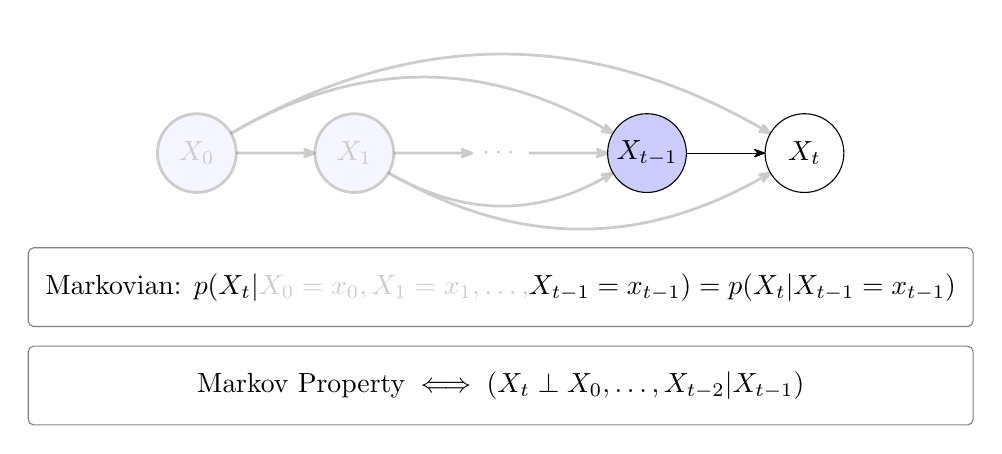
\begin{tikzpicture}
    \begin{scope}[
        opacity=0.2,
        transparency group]
        \node[observed rv] (X0) {$X_0$};
        \node[observed rv, right=of X0] (X1) {$X_1$};

        \node[right=of X1] (dots1) {$\cdots$};
    \end{scope}


    \node[observed rv, right=of dots1] (Xt-1) {$X_{t-1}$};
    \node[unobserved rv, right=of Xt-1] (Xt) {$X_{t}$};

    % \node[right=of Xt] (dots2) {$\cdots$};

    % \node[observed rv, right=of dots2] (XT-1) {$X_{T-1}$};
    % \node[unobserved rv, right=of XT-1] (XT) {$X_{T}$};

    \begin{scope}[
        opacity=0.2,
        transparency group]
        \draw[arrow, ->] (X0) to (X1);
        \draw[arrow, ->] (X1) to (dots1);
        \draw[arrow, ->, bend left] (X0) to (Xt);
        \draw[arrow, ->, bend left] (X0) to (Xt-1);

        \draw[arrow, ->, bend right] (X1) to (Xt);
        \draw[arrow, ->, bend right] (X1) to (Xt-1);

        \draw[arrow, ->] (dots1) to (Xt-1);
    \end{scope}
    \draw[arrow, ->] (Xt-1) to (Xt);
    % \draw[arrow, ->] (Xt) to (dots2);
    % \draw[arrow, ->] (dots2) to (XT-1);
    % \draw[arrow, ->] (XT-1) to (XT);




    \node[formula, below=1cm of dots1] (formula1) {Markovian:  $p(X_t| {\blendcolors*{!20}\color{black} X_0=x_0, X_1=x_1, \dots,} X_{t-1}=x_{t-1})= p(X_t| X_{t-1}=x_{t-1})$};

    \node[formula, below=0.25cm of formula1] (formula2) {$\text{Markov Property} \iff (X_t \perp X_0, \dots, X_{t-2} | X_{t-1})$};
\end{tikzpicture}
\end{document}